\label{results:umbrella}
% TODO: swap following sentences, start with importance of the patch
In order to understand the falling of FAK onto the membrane the free energy profile of the binding of the basic patch to \pip{} was investigated. Since this binding is the main contact between FAK and the membrane in our model, a short report on the results is given at this point.\\
The profiles are obtained from setup 2. The reaction coordinate is the z component of the COM distance between \pip{} and the protein fragment. For each forcefield, C36, \martini{} and \martini{} with PW, the average profile out of the five copies together with the standard deviation can be found in \autoref{umbrella:profiles}. The free energy profiles were shifted to be zero on average in the range $6\,\si{\nano\metre} \le z \le 7\,\si{\nano\metre}$.\\
%
%
%
\begin{figure}[hb]
	\centering
	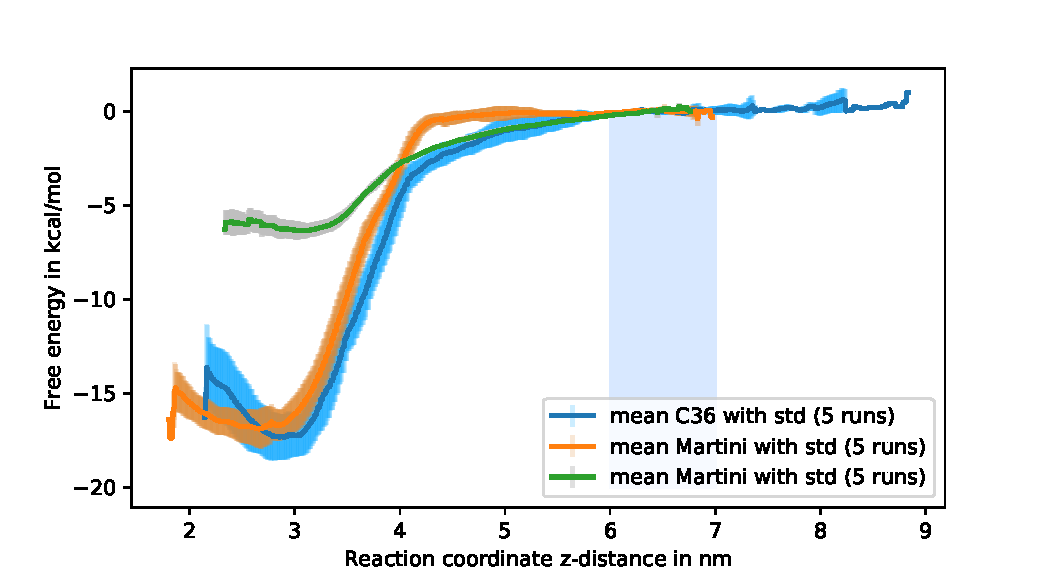
\includegraphics[width=.8\textwidth]{figures/results/umbrella}
	\nicecaption{Free energy profile of basic patch}{For each forcefield the average and standard deviation of the five copies is presented.}
	\label{umbrella:profiles}
\end{figure}
%
%
%
\\
%TODO: make c small in plot!
Both force fields, C36 and \martini{}, show a similar energy depth of $\approx 17 \si{\kilo cal/\mole}$ and a similar slope between $3\,\si{\nano\metre} \le z \le 4\,\si{\nano\metre}$.
% TODO: there is a small difference, ..., maybe more sampling to see if there is really a distance.
% TODO: range for value $4.2$
Certainly, \martini{} shows systematically more shallow wells than the all atom simulation. This can be attributed to the proposed underestimation of electrostatic forces due to the non-polar water beads (see \autoref{subsub:coarsegraining}). The difference at $z = 4.2\,\si{\nano\metre}$ originates from the different treatment of long-range electrostatics: whereas \martini{} uses a cut-off radius, C36 uses PME.\\ %TODO: maybe force switch function in martini? what about the kink in C36?
Also \martini{} with PW uses PME for long-range electrostatic interactions, and indeed it fits much better to the C36 profile for larger distances. However, the binding strength is crucially underestimated in Martini with PW.\\
The extent to which \martini{} reproduces the results from all-atom simulations is remarkable, even though the parameters for \martini{} were obtained from free energy calculations (see \autoref{subsub:coarsegraining}).\\
\\
In the used starting configurations, the proteins are already bound to \pip{}. Therefore, a correct binding strength and the shape near the minimum is of larger interest than a correct sampling of farther distances. In addition, \martini{} with PW required a much higher computational effort. Hence, we consider only the standard water model in the following simulations.
